\documentclass[../main.tex]{subfiles}


\usepackage{nopageno} %Seitenzahlen auf richtiger Seite 

\usepackage[left=2cm, right=2cm, top=2cm, includehead, includefoot, headheight=17pt]{geometry}

\usepackage[utf8x]{inputenc}
\usepackage[english]{babel}
\usepackage{amsmath,amssymb,amsthm}
\usepackage{framed}
\usepackage{wasysym}
\usepackage[T1]{fontenc} %Silbentrennung 
\usepackage{color} %Farbe
\usepackage{graphicx}
\usepackage{float}%Grafik am gleichen Ort plazieren
%pdf. png. einfach eingliedern
\usepackage{subfigure} %Grafiken nebeneinander
\usepackage{pdfpages}
\usepackage{ulem} 	%\uuline{urgent}    % doppelt unterstreichen
%\uwave{boat}      % unterschlängeln
%\sout{wrong}       % durchstreichen
%\xout{removed}     % ausstreichen mit //////.

\usepackage{tikz}
\usetikzlibrary{trees}
\usetikzlibrary{plotmarks}
\usetikzlibrary{angles,quotes,babel}
\usetikzlibrary{shadings}
\usetikzlibrary{patterns}
\usetikzlibrary{matrix}
\usetikzlibrary{arrows}
\usetikzlibrary{calc}

\usepackage{pgfplots}
\usepackage{pgf-pie}
\pgfplotsset{compat=1.10}
\usepgfplotslibrary{statistics}
\usepgfplotslibrary{fillbetween}

\usepackage{tkz-euclide}
\usepackage{enumerate}
\usepackage{stmaryrd}
\usepackage{tabularx}
\usepackage{wrapfig}
\usepackage{epsdice}
\usepackage{multirow}
\usepackage{rotating}
\usepackage{pdflscape}
\usepackage{fancyhdr}

\pagestyle{fancy} %eigener Seitenstil
\fancyhf{} %alle Kopf- und Fußzeilenfelder bereinigen
\fancyhead[L]{} %Kopfzeile links
\fancyhead[C]{} %zentrierte Kopfzeile
\fancyhead[R]{} %Kopfzeile rechts
\renewcommand{\headrulewidth}{0.4pt} %obere Trennlinie
\fancyfoot[C]{\thepage} %Seitennummer
\renewcommand{\footrulewidth}{0.4pt} %untere Trennlinie

% Number spaces 
\newcommand{\CC}{\ensuremath{\mathbb{C}}}
\newcommand{\RR}{\ensuremath{\mathbb{R}}}
\newcommand{\QQ}{\ensuremath{\mathbb{Q}}}
\newcommand{\ZZ}{\ensuremath{\mathbb{Z}}}
\newcommand{\NN}{\ensuremath{\mathbb{N}}}
\newcommand{\LL}{\ensuremath{\mathbb{L}}}
\newcommand{\DD}{\ensuremath{\mathbb{D}}}
\newcommand{\WW}{\ensuremath{\mathbb{W}}}

%draw chemestry molecules 
\usepackage{chemfig} % https://mirror.ox.ac.uk/sites/ctan.org/macros/generic/chemfig/

\newcommand\vv[1]{%
	\begin{tikzpicture}[baseline=(arg.base)]
		\node[inner xsep=0pt] (arg) {$#1$};
		\draw[line cap=round,line width=0.45,->,shorten >= 0.2pt, shorten <= 0.7pt] (arg.north west) -- (arg.north east);
	\end{tikzpicture}%
} %command will render \vv{x} with an arrow aboth 

\renewcommand{\labelenumi}{\roman{enumi})}

\DeclareMathOperator{\ggT}{ggT}
\DeclareMathOperator{\sign}{sign}

%sections
\theoremstyle{plain}
\newtheorem{Thm}{Theorem}[section]
\newtheorem{Def}[Thm]{Definition}
\newtheorem{Prop}[Thm]{Proposition}

\theoremstyle{definition}
\newtheorem{lemma}[Thm]{Lemma}
\newtheorem{corollary}[Thm]{Corollary}
\newtheorem{claim}[Thm]{Claim}
\newtheorem{Proof}[Thm]{Proof}
\newtheorem{Ex}[Thm]{Example}

\newtheorem{Exercise}{ex}[section] %follow proper enum
\newtheorem{ex}[Exercise]{Exercise}
\newtheorem{Solution}{sol}[section]
\newtheorem{sol}[Solution]{Solution}

\theoremstyle{remark}
\newtheorem{remark}[Thm]{Remark} % follows thm enum

\newtheorem{comment}{Comment}[section] %follow comment enum
\newtheorem{notation}[comment]{Notation}
\newtheorem{reasoning}[comment]{Reasoning}
\newtheorem{Intpr}[comment]{Interpretation}

%some premmade with title (uterwise use \textbf{Title} ...)
\newenvironment{ThmWithTitle}[1]{%
	\begin{Thm}[\textbf{#1}]}{\end{Thm}}
\newenvironment{PropWithTitle}[1]{%
	\begin{Prop}[\textbf{#1}]}{\end{Prop}}
\newenvironment{ExWithTitle}[1]{%
	\begin{Ex}[\textbf{#1}]}{\end{Ex}}
\newenvironment{DefWithTitle}[1]{%
	\begin{Def}[\textbf{#1}]}{\end{Def}}
\newenvironment{RemarkWithTitel}[1]{%
	\begin{remark}[\textbf{#1}]}{\end{remark}}

%format of paragraph 
\renewcommand\paragraph{\@startsection{paragraph}{4}{\z@}%
	{-2.5ex\@plus -1ex \@minus -.25ex}%
	{1.25ex \@plus .25ex}%
	{\normalfont\normalsize\bfseries}}
\makeatother
\setcounter{secnumdepth}{4} % how many sectioning levels to assign numbers to
\setcounter{tocdepth}{4}    % how many sectioning levels to show in ToC

\newcounter{row} 
\renewcommand\therow{\alph{row}} %hier a,b,c etc. def und mit therow abrufbar

\newenvironment{aufz}
{\setcounter{row}{0}%
	\par\noindent\tabularx{\linewidth}[t]
	{\cdot{20}{>{\stepcounter{row}\makebox[1.5em][l]{\therow)\hfill}}X}} %bis max 20 Elemente nebeinander
}
{\endtabularx}


%biblio
\usepackage[]{biblatex}
\addbibresource{referenzenma.bib} 

%glossary
\usepackage{glossaries}
\usepackage{import}


\usepackage{rotating} % Include this package in the preamble

\newglossaryentry{necrosis}{
	name=necrosis,
	description={A form of uncontrolled cell death resulting from acute cellular injury, leading to the rupture of the plasma membrane and inflammation of the surrounding tissue. Cell looks like it exploded}
}

\newglossaryentry{apoptosis}{
	name=apoptosis,
	description={A regulated, energy-dependent form of programmed cell death characterized by cell shrinkage, DNA fragmentation, membrane blebbing, and the absence of inflammation}
}

\newglossaryentry{XIAP}{
	name=XIAP,
	description={X-linked inhibitor of apoptosis protein; a member of the IAP family that binds to and inhibits caspases, particularly caspase-3, -7, and -9, thereby blocking apoptosis}
}

\newglossaryentry{FLIP}{
	name=FLIP,
	description={FLICE-like inhibitory protein; a regulator that inhibits caspase-8 activation at the death-inducing signaling complex (DISC), thereby preventing the initiation of extrinsic apoptosis}
}

\newglossaryentry{initiatorcaspases}{
	name=initiator caspases,
	description={A class of caspases (e.g., caspase-8 and caspase-9) that are activated early in the apoptotic signaling cascade and initiate apoptosis by activating executioner caspases}
}

\newglossaryentry{executionercaspases}{
	name=executioner caspases,
	description={A class of caspases (e.g., caspase-3 and caspase-7) that carry out apoptosis by cleaving a wide range of cellular substrates, leading to controlled cellular dismantling}
}

\newglossaryentry{CAD}{
	name=CAD,
	description={Caspase-Activated DNase; an endonuclease that, upon release from its inhibitor iCAD by executioner caspases, cleaves chromosomal DNA during apoptosis, producing characteristic nucleosome-sized fragments}
}

\newglossaryentry{caspases}{
	name=caspases,
	description={Caspases are a family of proteases that use a cysteine residue in their active site and specifically cleave peptide bonds after aspartic acid residues in substrate proteins}
}

\newglossaryentry{fasreceptor}{
	name=Fas receptor,
	description={A cell-surface death receptor also known as CD95 or APO-1, part of the TNF receptor family. Upon binding its ligand (FasL), it triggers the extrinsic apoptotic signaling pathway}
}

\newglossaryentry{fadd}{
	name=FADD,
	description={Fas-Associated protein with Death Domain; an adaptor protein that binds to death receptors such as Fas. It recruits and activates initiator caspases (e.g., caspase-8), playing a key role in the extrinsic apoptotic pathway}
}

\newglossaryentry{deathsreceptors}{
	name=cell-surface death receptors,
	description={Transmembrane proteins that belong to the TNF (tumor necrosis factor) receptor family and can initiate apoptosis when bound by their ligands. Examples include Fas receptor and TNF receptor}
}

\newglossaryentry{tnf}{
	name=TNF,
	description={Tumor Necrosis Factor; a cytokine involved in systemic inflammation. It can bind to TNF receptors, including death receptors, and promote cell death or survival depending on cellular context}
}

\newglossaryentry{disc}{
	name=DISC,
	description={Death-Inducing Signaling Complex; a multiprotein complex formed upon activation of cell-surface death receptors (such as Fas or TNF receptors). It includes adaptor proteins like FADD and initiator caspases (e.g., caspase-8), and initiates the extrinsic apoptosis pathway}
}

\newglossaryentry{cytochromec}{
	name=Cytochrome~c,
	description={A mitochondrial protein that, when released into the cytosol, helps activate apoptosis by binding Apaf1}
}

\newglossaryentry{apaf1}{
	name=Apaf1,
	description={Apoptotic protease-activating factor 1; binds cytochrome~c and forms the apoptosome to activate caspase-9}
}

\newglossaryentry{apoptosome}{
	name=Apoptosome,
	description={A multiprotein complex formed by Apaf1 and cytochrome~c that activates initiator caspase-9}
}

\newglossaryentry{bcl2family}{
	name=Bcl-2~family,
	description={A group of proteins that regulate mitochondrial outer membrane permeabilization and apoptosis}
}

\newglossaryentry{bax}{
	name=Bax,
	description={A pro-apoptotic Bcl-2 family protein that promotes cytochrome~c release from mitochondria}
}

\newglossaryentry{bak}{
	name=Bak,
	description={A pro-apoptotic Bcl-2 family member that cooperates with Bax to permeabilize the mitochondrial membrane}
}

\newglossaryentry{BH3domain}{
	name={BH3 domain},
	description={A short conserved sequence found in Bcl-2 family proteins. It enables pro-apoptotic proteins to bind to and inhibit anti-apoptotic Bcl-2 proteins, promoting apoptosis}
}


\newglossaryentry{survivalfactor}{
	name={survival factor},
	description={An extracellular signaling molecule that promotes cell survival by inhibiting apoptosis. Survival factors typically act by activating cell-surface receptors, which trigger intracellular pathways that suppress pro-apoptotic proteins}
}

\newglossaryentry{IAP}{
	name={IAP},
	description={Short for \textit{Inhibitor of Apoptosis Protein}. A family of proteins that inhibit caspase activity and thereby block apoptosis. IAPs typically contain BIR (baculovirus IAP repeat) domains and may also promote the degradation of caspases via ubiquitylation}
}

\newglossaryentry{eat-me-signal}{
	name={Eat-me signal},
	description={A molecular marker exposed on the surface of apoptotic cells that signals phagocytes to recognize and engulf them. A common eat-me signal is phosphatidylserine (PS), a phospholipid normally located on the inner leaflet of the plasma membrane but externalized during apoptosis to promote clearance of dying cells.}
}



\makeglossaries


\begin{document}
	
\section{Cell Death}



\subsection{Apoptosis - Programmed cell death}
The growth, development, and maintenance of multicellular organisms depend not only on the production of cells but also on mechanisms to destroy them. The maintenance of tissue size, for example, requires that cells die at the same rate as they are produced. Moreover cells have to die when thex become damaged or infected, ensuring that they are removed before they threaten the health of the organism.\\
\indent In most cases this is not radon but rather precisely controlled, we speek of \textbf{programmed cell death}. The most prominent process is called \textbf{apotosis}, which can be intrinsic regulated through the mitochondria or extrinsic regulated through cell signaling. There are also other processes, that won't be lookt at, but just for completion: Phagocytosis, Ferroptosis, Necroptosis (similar to necrosis but controlled), Pyroptosis (during infection), and Cornification (skin keratinization). \\
\indent Nevertheless the cell death can also occure unprogrammed, we then speak of \textbf{unprogrammed cell death}, a process is \textbf{\gls{necrosis}} (accidental cell death). In most cases necrosis is caused by \textbf{energy depletion}. This often happens to \textbf{tumor cells}, as a tumor grows randomly and cells can get cut of from supplies, which leads to accidental cell death. \\
\indent Cells \textbf{dying by necrosis} swell and \textbf{burst, spilling} their contents over their neighbors and eliciting an inflammatory response. Therefore cells that have died by necrosis look like they \textbf{exploded. See fig. \ref{necrosis}}

\begin{figure}[H]
	\centering
	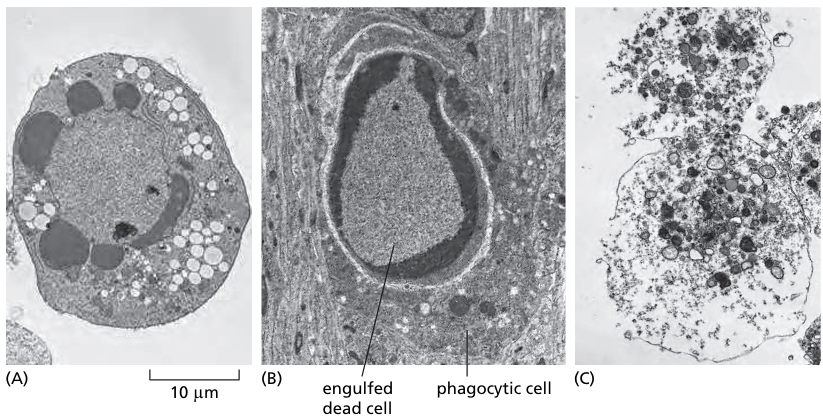
\includegraphics[width = 0.7\textwidth]{1}
	\caption{Two distinct forms of cell death. Apoptosis (A \& B), Necrosis (C)}
	\label{necrosis}
\end{figure}

In contrast, Cells \textbf{dying by \gls{apoptosis}} undergo characteristic morphological changes \textbf{(See fig \ref{necrosis})}. They \textbf{shrink and condense}, the cytoskeleton collapses, the nuclear envelope disassembles, and the nuclear chromatin condenses and breaks up into fragments. The cell surface often bulges outward and, if the cell is large, it breaks up into membrane-enclosed fragments called \textbf{apoptotic bodies}. The surface of the cell or apoptotic bodies becomes chemically altered, so that a neighboring cell or a macrophage rapidly engulfs them, before they can spill their contents, through \textbf{phagocytosis. (See fig. \ref{apoptosis-steps})} In this way, the cell dies neatly and is rapidly cleared away, without causing a damaging inflamatory response. \\
\\
\indent Basically a \textbf{cell needs to be convinced not to die}. Therefore for cell death to happen we deactivate a regulator of cell death, leading to cell death. \\
When apoptosis is triggered (\textbf{\gls{initiatorcaspases} (9 or 8)}) the commitment to die is still \textbf{reversible} (for example DNA repair occurs). The intrinsic and extrinsic pathway then converge to the \textbf{\gls{executionercaspases} (3, 7)}. Once they are activated the cell is committed to apoptosis. (See fig. \ref{apoptosis-steps}) Note the role of \textbf{\gls{XIAP}} and \textbf{\gls{FLIP}} that block caspases and are essential to ensure tight \textbf{all-or-nothing regulation}. 
\begin{figure}[H]
	\centering
	\subfigure[]{
		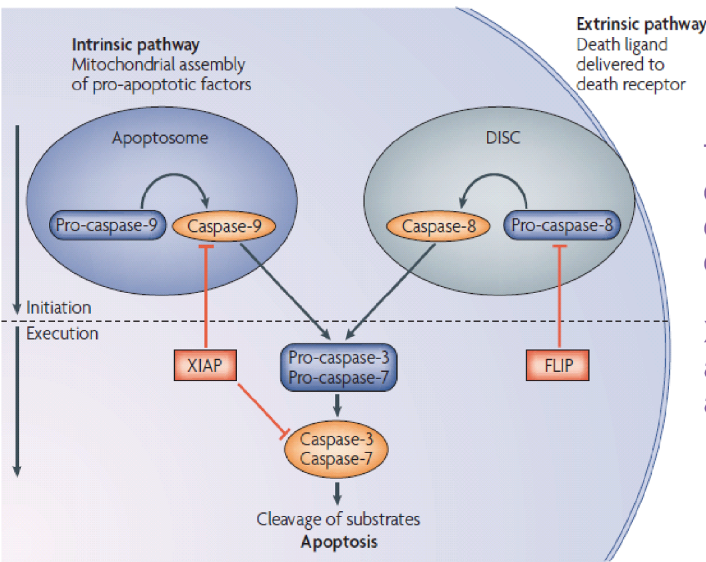
\includegraphics[width = 0.45 \textwidth]{4}
	}
	% Second subfigure
	\subfigure[]{
		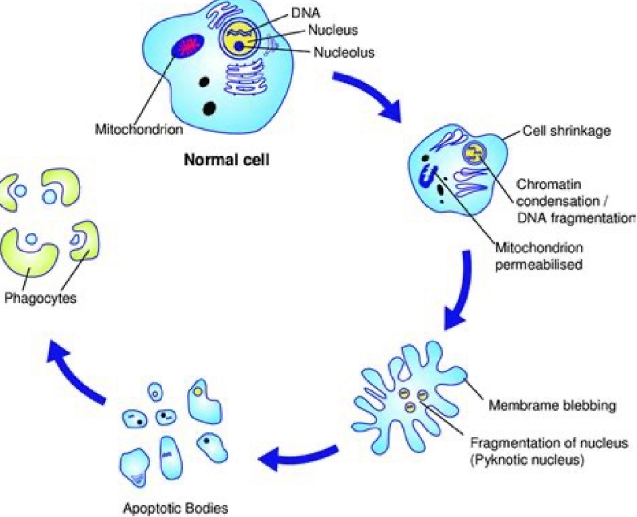
\includegraphics[width = 0.5 \textwidth]{3}
	}
	\caption{Steps of Apoptosis}
	\label{apoptosis-steps}
\end{figure}

\begin{RemarkWithTitel}{DNA fragmentation during apoptosis.}
	During apoptosis, the DNA of a dying cell is systematically fragmented by a \textbf{nuclease called \gls{CAD} (Caspase-Activated DNase)}. Under normal conditions, CAD is kept inactive through binding to its \textbf{inhibitor, iCAD}. However, when e\textbf{xecutioner caspases are activated during apoptosis, they cleave iCAD}, releasing CAD to cut DNA between nucleosomes. This results in DNA fragments that appear as a distinctive "ladder" pattern when separated by gel electrophoresis. The presence of these DNA fragments can also be visualized in tissues using the TUNEL assay, which labels exposed DNA ends with fluorescent markers, highlighting apoptotic cells. \textbf{See fig. \ref{DNAfragmentation}}
	\begin{figure}[H]
		\centering
		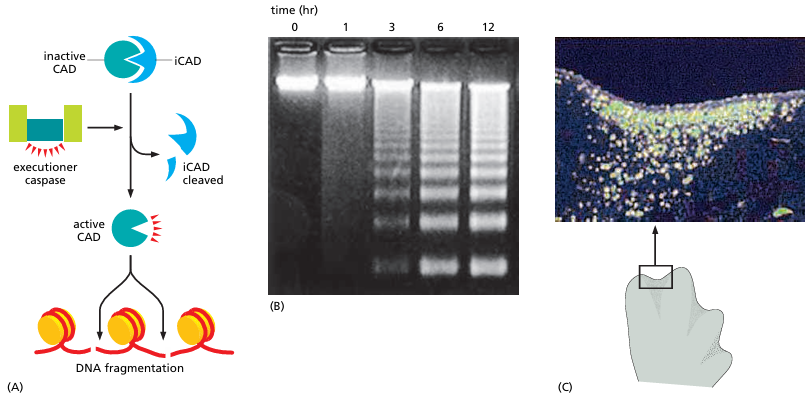
\includegraphics[width = \textwidth]{6}
		\caption{DNA fragmentation during apoptosis.}
		\label{DNAfragmentation}
	\end{figure}
\end{RemarkWithTitel}


\begin{RemarkWithTitel}{Dead cell removal by Efferocytosis}
	Elimination of dead cell bodies is important to\textbf{prevent the release of intracellular} content that may function as damage-associated molecular patterns to \textbf{activate an inflammatory} response and possibly lead to \textbf{autoimmunity}.
\end{RemarkWithTitel}


\begin{RemarkWithTitel}{Apoptosis plays an important role during development of many tissues.}
	Cell death helps sculpt \textbf{hands and feet during embryonic development}: they start out as spade-like structures, and the individual digits separate only as the cells between them die. See fig. \ref{DNAfragmentation}(c)\\
	\indent Moreover, apoptosis also functions as a \textbf{quality-control} process in development, eliminating cells that are abnormal, misplaced, nonfunctional, or potentially dangerous to the animal. Striking examples occur in the vertebrate adaptive immune system, where apoptosis eliminates \textbf{developing T and B lymphocytes} that either fail to produce potentially useful antigen-specific receptors or produce self-reactive receptors 
	that make the cells potentially dangerous. 
\end{RemarkWithTitel}


\subparagraph{Caspases}
\gls{caspases} are a\textbf{ family of proteases that use a cysteine residue in their active site and specifically cleave peptide bonds after aspartic acid residues} in substrate proteins. They play essential roles in apoptosis, inflammation, and cell differentiation.\\
\\
\indent An \textbf{\gls{initiatorcaspases}} contains a protease domain in its carboxy-terminal 
region and a small protein interaction domain near its amino terminus. It is \textbf{initially 
made in an inactive}, monomeric form, sometimes called \textbf{procaspase}. \textbf{Apoptotic signals trigger the assembly} of adaptor proteins carrying multiple binding sites for the caspase amino-terminal domain. Upon binding to the adaptor proteins, the \textbf{initiator caspases dimerize and are thereby activated}, leading to cleavage of a specific site in their protease domains. \\
\indent Each protease domain is then rearranged into a large and small subunit. In some cases 
(not shown in fig. \ref{caspase-activation}), the adaptor-binding domain of the initiator caspase is also cleaved (see. fig fig. \ref{caspase-activation}). \\
\indent \textbf{\gls{executionercaspases} are initially formed as inactive dimers}. Upon \textbf{cleavage at a site in the protease domain by an initiator caspase - this is the point of no return - }, the executioner caspase dimer undergoes an activating conformational change. The executioner caspases then cleave a variety of key proteins, leading to the controlled death of the cell. 

\begin{figure}[H]
	\centering
	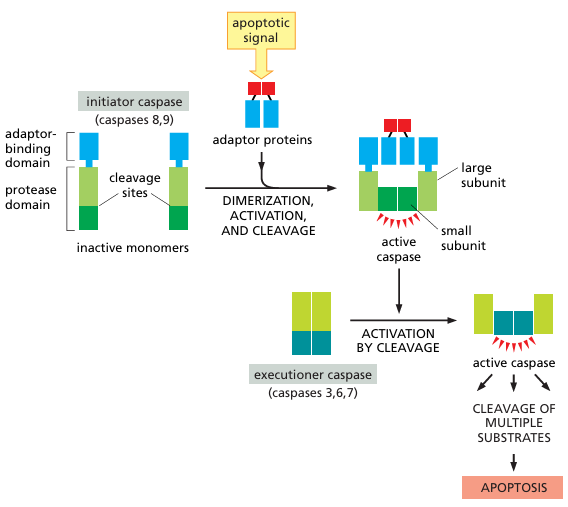
\includegraphics[width = 0.55\textwidth]{2}
	\caption{Caspase activation during apoptosis.}
	\label{caspase-activation}
\end{figure}

\paragraph{Extrinsic Pathway of Apoptosis}

In the extrinsic pathway the cell death is \textbf{triggered by an other cell}. Extracellular signal proteins binding to \textbf{\gls{deathsreceptors}} trigger apoptosis. Death receptors are transmembrane proteins containing an extracellular ligand-binding domain, a single transmembrane domain, and an intracellular death domain, which is required for the receptors to activate the apoptotic program. The receptors are homotrimers and belong to 
the \textbf{tumor necrosis factor (TNF) receptor family}, which includes a receptor for \textbf{\gls{tnf}} itself and the \textbf{\gls{fasreceptor}}.\\
\\
\indent A well understood example is the \textbf{FAS receptor}. Trimeric Fas ligands on the surface of a killer lymphocyte interact with trimeric Fas receptors on the surface of the 
target cell, leading to clustering of several ligand-bound receptor trimers (only one 
trimer is shown in fig. \ref{Fas-shit}). \textbf{Receptor clustering activates death domains} on the receptor tails, which \textbf{interact with similar domains on the adaptor protein \gls{fadd}} (FADD stands for Fas-associated death domain). Each FADD protein then recruits an initiator caspase (caspase-8) via a death effector domain on both FADD and the caspase, forming a \textbf{death-inducing signaling complex (DISC)}. \\
\indent Within the \textbf{\gls{disc}}, two adjacent initiator caspases interact and cleave one another to form an activated protease dimer, which then cleaves itself in the region linking the protease to the death effector domain. This \textbf{stabilizes and releases the active caspase dimer into the cytosol}, where it activates executioner caspases by cleaving them.

\begin{figure}[H]
	\centering
	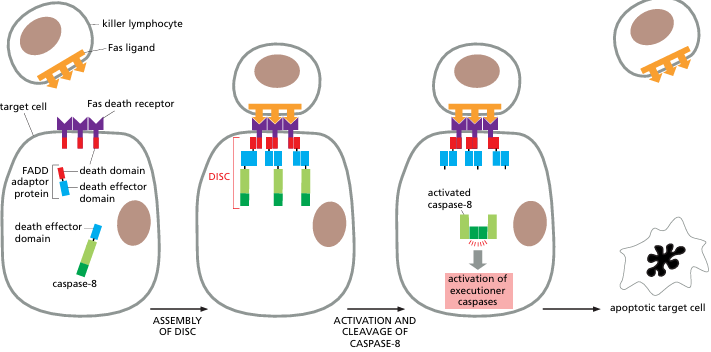
\includegraphics[width = 0.9\textwidth]{7}
	\caption{The extrinsic pathway of apoptosis activated through Fas death receptors.}
	\label{Fas-shit}
\end{figure}

\paragraph{Intrinsic Pathway of Apoptosis}
Cells can also activate their apoptosis program from inside the cell, often in response to stresses, such as DNA damage, or in response to developmental signals (ex. Withdrawal of growth factors). \textit{Some of these signals may technically  be on the basis of environmental factors (UV). But the intrinsic property of the cell induces apoptosis and not an other cell.}\\
\indent The intrinsic pathway is also called the \textbf{mitochondrial pathway} because it is triggered by the\textbf{ release of cytochrome c from the intermembrane space into the cytosol}.
\begin{figure}[H]
	\centering
	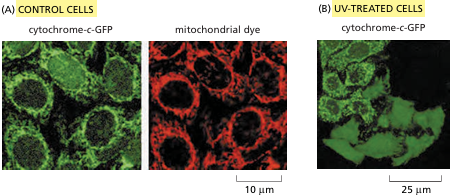
\includegraphics[width = 0.9\textwidth]{9}
	\caption{Release of cytochrome c from mitochondria in the intrinsic pathway of apoptosis.}
\end{figure}

Once in the cytosol, cytochrome c binds to \textbf{\gls{apaf1}} (apoptotic protease activating factor-1), triggering it to assemble into a large, heptameric complex called the \textbf{\gls{apoptosome}}. This structure recruits and activates caspase-9 via its \textbf{\gls{card} domains} (caspase recruitment domains). Activated caspase-9 then initiates a cascade by activating downstream executioner caspases, leading to controlled cell death. \textbf{See fig. \ref{intrinsic-pathway}}

\begin{figure}[H]
	\centering
	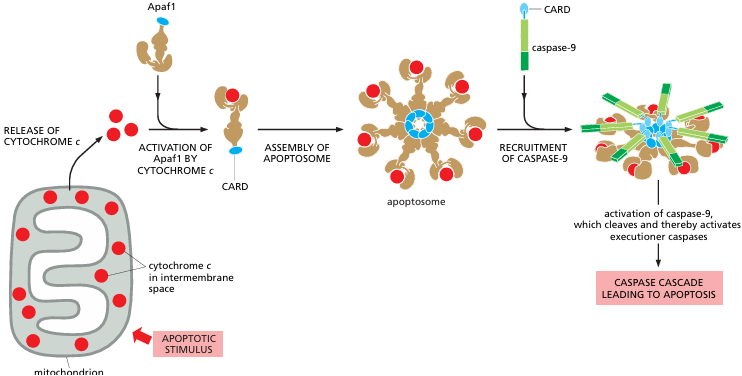
\includegraphics[width = 0.9\textwidth]{8}
	\caption{The intrinsic pathway of apoptosis.}
	\label{intrinsic-pathway}
\end{figure}

\begin{RemarkWithTitel}{\gls{cytochromec} is important for cell life and also cell death. That fucker!}
	It is all \textbf{about its location}: 
	\begin{itemize}
		\item For the cell’s life: cytochrome c, inside the \textbf{mitochondrial interspace}, is an indispensable \textbf{electron carrier protein} for the mitochondrial electron-transport chain (transports electrons between III and IV)
		
		\item For the cell’s death: if \textbf{released in the cytosol}, cytochrome c is converted into a pro-apoptotic molecule. It will bind \textbf{Apaf-1} to trigger the \textbf{activation of procaspase- 9}, altogether forming the \textbf{“apoptosome” complex}, which will then \textbf{activate caspase-3  and cause apoptosis}.
	\end{itemize}
\end{RemarkWithTitel}

\subparagraph{The Bcl-2~family}
The intrinsic pathway of apoptosis is tightly regulated by the \textbf{\gls{bcl2family} of proteins, which control the release of cytochrome c} and other mitochondrial proteins that trigger cell death. These proteins fall into three groups (See fig. \ref{Bcl-2-family}):
\begin{itemize}
	\item \textbf{Anti-apoptotic proteins} (e.g., Bcl2, BclXL): prevent apoptosis by inhibiting pro-apoptotic proteins.
	
	\item \textbf{Pro-apoptotic effector proteins} (e.g., \textbf{\gls{bax}, \gls{bak}}): promote apoptosis by forming oligomers in the mitochondrial membrane to release cytochrome c.
	
	\item \textbf{BH3-only proteins} (e.g., Puma, Noxa, Bid): act as sensors of apoptotic stimuli, inhibiting anti-apoptotic proteins and/or activating Bax and Bak.
\end{itemize}
Note that the \textbf{\gls{BH3domain}} is the only BH domain shared by all Bcl2 family members. It meadiates the direct interactions between pro-apoptotic and andt-apoptotic family members. 

\begin{figure}[H]
	\centering
	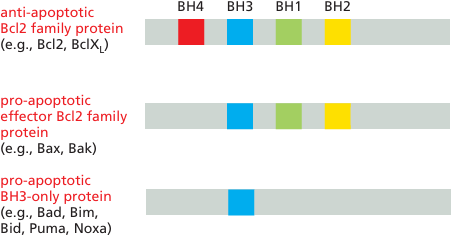
\includegraphics[width = 0.5\textwidth]{10}
	\caption{The three classes of Bcl2 family proteins.}
	\label{Bcl-2-family}
\end{figure}

\indent The balance between pro- and anti-apoptotic Bcl2 family members determines whether a cell undergoes apoptosis. In response to stress (e.g., DNA damage), BH3-only proteins are activated—often through p53—and \textbf{inactivated anti-apoptotic proteins}, enabling \textbf{Bax and Bak to permeabilize the mitochondria}.\\
\indent Furthermore, the extrinsic pathway of apoptosis can activate the intrinsic pathway via the BH3-only protein Bid, which is cleaved by caspase-8, amplifying the apoptotic response.

\begin{figure}[H]
	\centering
	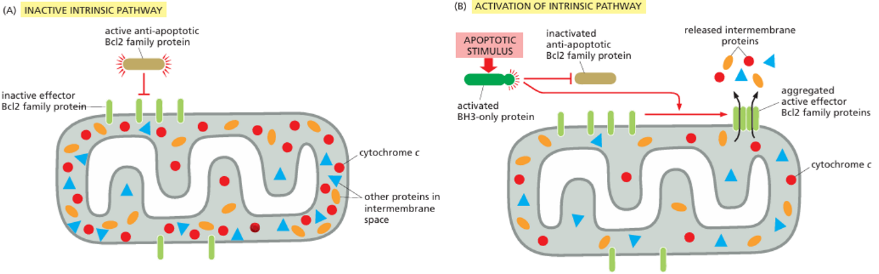
\includegraphics[width = 0.9\textwidth]{11}
	\caption{How pro-apoptotic BH3 only and anti-apoptotic Bcl2 family proteins regulate the intrinsic pathway of apoptosis.}
\end{figure}


\paragraph{Overview Intrinsic and Extrinsic}

\begin{figure}[H]
	\centering
	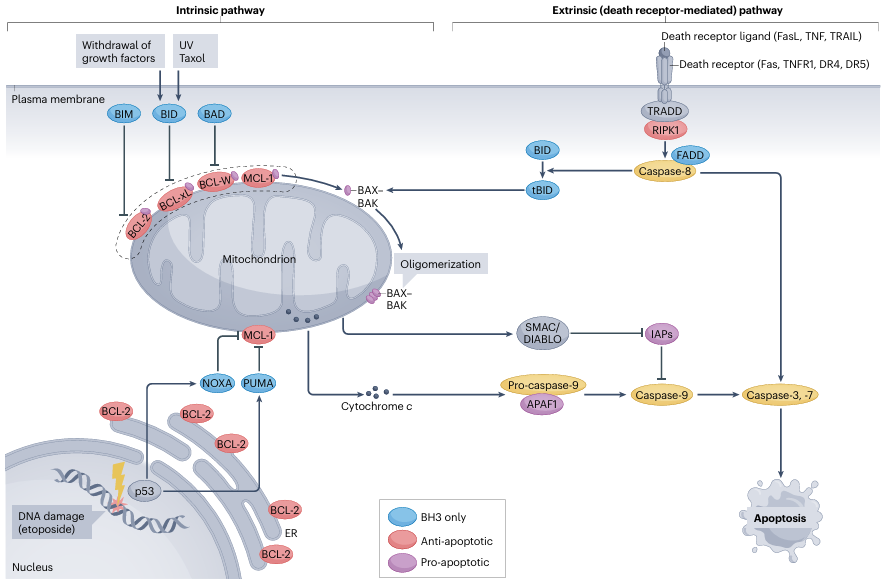
\includegraphics[width = \textwidth]{5}
	\caption{Intrinsic and extrinsic apoptosis.}
\end{figure}

\subsubsection{Inhibiting Apoptosis}
\indent Cells strictly regulate apoptosis, especially the caspase cascade, to prevent accidental cell death. One layer of control is provided by \textbf{\gls{IAP}s (Inhibitors of Apoptosis Proteins}), which inhibit active caspases using their BIR (\textit{baculovirus IAP repeat}) domains. \\
\indent Some IAPs also tag caspases for destruction via ubiquitylation. In insects like Drosophila, apoptosis is tightly controlled by a \textbf{balance between IAPs and anti-IAPs} (e.g. Reaper, Grim, and Hid), which block IAPs and promote cell death. In mammals, mitochondrial release of anti-IAPs (like Smac/Diablo and Omi) helps relieve IAP inhibition during intrinsic apoptosis, but their role appears less essential than in flies.\\
\\
\indent Additionally, \textbf{extracellular \gls{survivalfactor}} are crucial in preventing apoptosis. These signals, such as growth factors or neurotrophins, bind to cell-surface receptors and inhibit the apoptotic machinery. They are \textbf{3 main ways how they act (see. fig \ref{survival-factors})}: 
\begin{enumerate}
	\item[(a)] \textbf{Upregulating anti-apoptotic Bcl2} family proteins (e.g. Bcl2, BclXL),
	\item[(b)] \textbf{Inhibiting pro-apoptotic BH3-only proteins} (e.g. Bad),
	\item[(c)] \textbf{Inactivating anti-IAPs} through phosphorylation (in Drosophila).
\end{enumerate}

\begin{figure}[H]
	\centering
	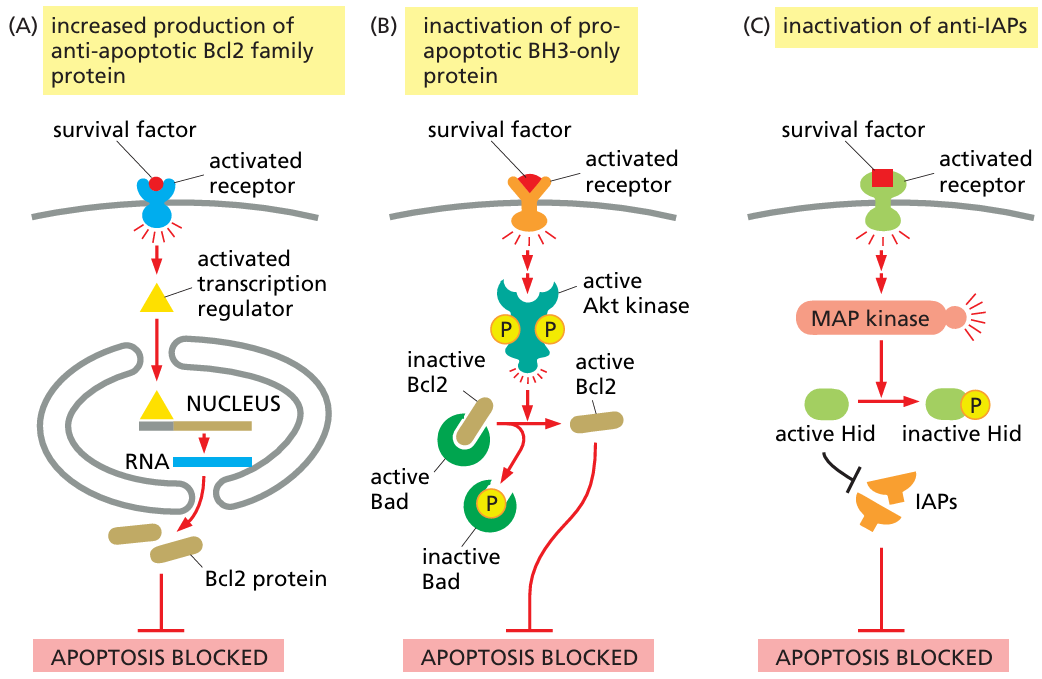
\includegraphics[width = 0.6\textwidth]{12}
	\caption{Three ways that extracellular survival factors can inhibit apoptosis.}
	\label{survival-factors}
\end{figure}
Cells, especially\textbf{ during development, rely on limited survival factors} from neighboring cells. For instance, neurons that fail to receive enough survival signals undergo apoptosis, which helps match neuron numbers to their target cells. See fig. \ref{Neurons-survival}
\begin{figure}[H]
	\centering
	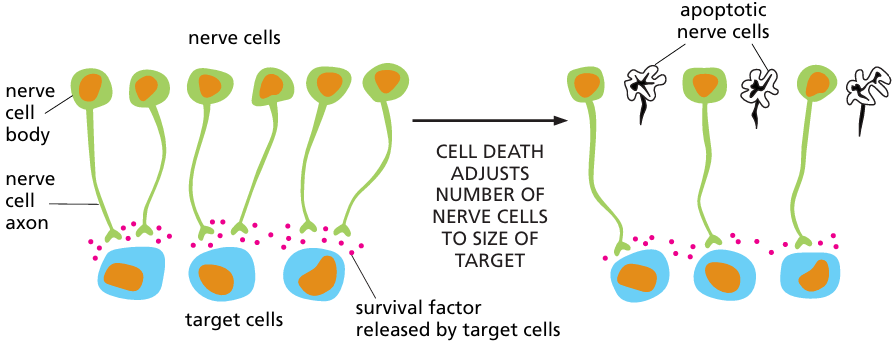
\includegraphics[width = 0.6\textwidth]{13}
	\caption{The role of survival factors and cell death in adjusting the number of developing nerve cells to the amount of target tissue.}
	\label{Neurons-survival}
\end{figure}


\begin{RemarkWithTitel}{Control over apoptosis}
	\textbf{Chemical inducers of dimerization (CIDs)} such as AP1903 or AP20187 can control apoptosis by \textbf{activating engineered proteins like inducible caspase-9}. When the CID is added, it binds to and dimerizes caspase-9, triggering its activation and initiating the apoptotic cascade. This system allows precise control over cell death in experimental or therapeutic settings.
\end{RemarkWithTitel}

\subsubsection{Identifying Apoptotic Cells}
Identifying apoptotic cells involves several complementary methods:
\begin{itemize}
	\item \textbf{Transmission electron microscopy} (TEM) allows visualization of characteristic morphological changes, such as cell shrinkage, chromatin condensation, and membrane blebbing.
	
	\item  At the molecular level, \textbf{DNA fragmentation} into nucleosome-sized fragments produces a distinctive "ladder" pattern detectable by gel electrophoresis.
	
	\item  Apoptosis is also confirmed by measuring \textbf{caspase activity}, often through \textbf{colorimetric assays} that detect cleavage of specific caspase substrates, indicating activation of these proteases.
	
	\item Additionally, release of \textbf{cytochrome c} from mitochondria into the cytosol is a hallmark of the intrinsic apoptotic pathway.
	
	\item  Finally, apoptotic cells expose \textbf{phosphatidylserine (PS)} on their outer membrane leaflet, which acts as an \textbf{\gls{eat-me-signal}} and can be detected using \textbf{annexin V staining}, aiding in the recognition and clearance of dying cells. \textit{Recall that PS is normally located on the inner leaflet of the plasma membrane but externalized during apoptosis to promote clearance of dying cells.}
\end{itemize}

\begin{figure}[H]
	\centering
	\subfigure[PS translocated to the outer membrane during apoptosis]{
		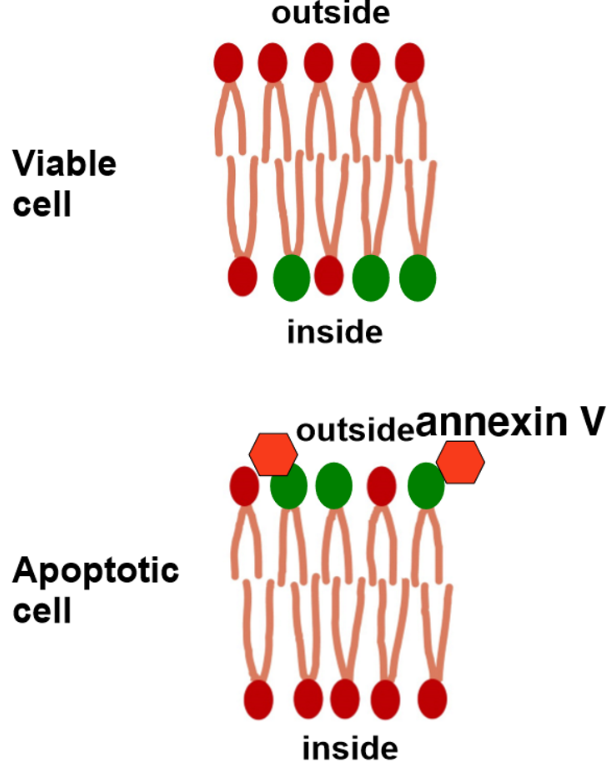
\includegraphics[width = 0.3 \textwidth]{15}
	}
	% Second subfigure
	\subfigure[External PS (PtdSer) "eat-me" signal]{
		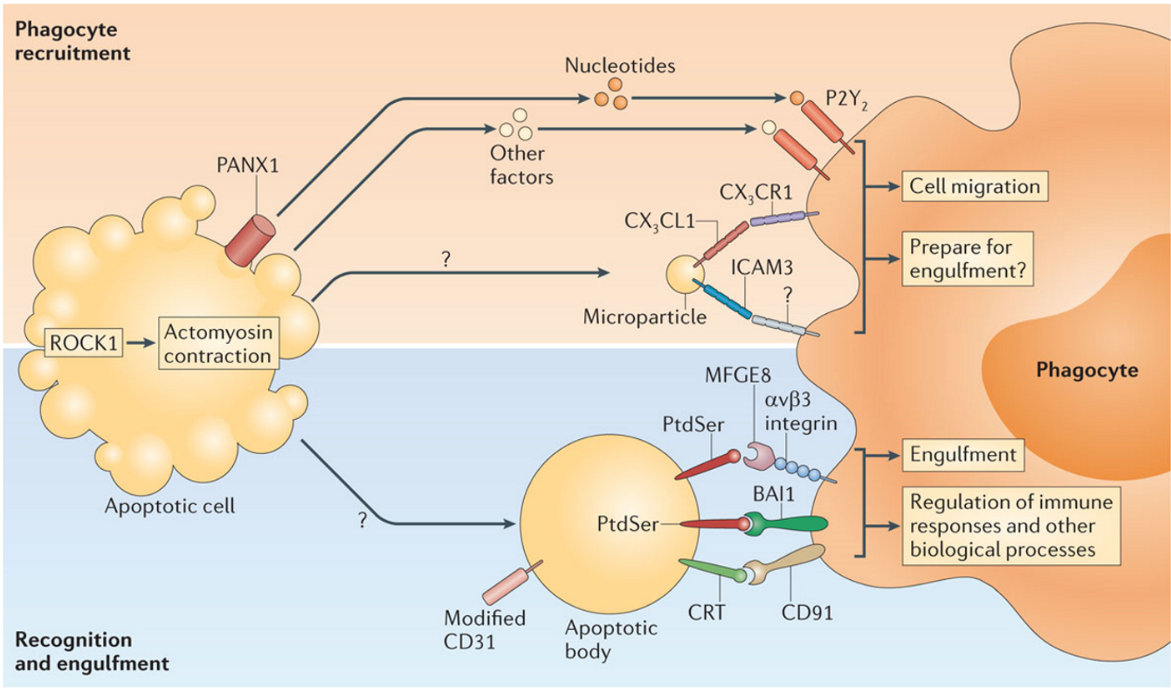
\includegraphics[width = 0.6 \textwidth]{14}
	}
	\caption{Detecting Apoptosis by marking external PS with Annexin V}
\end{figure}

\printglossaries

	
\end{document}